\chapter{Validación de la Implementación y Experimentos}\label{chapter:implementation}

En este capítulo, se detalla la implementación de la solución propuesta, analizando un caso de prueba detalladamente paso a paso.  En cada etapa de este caso de prueba, se describe el proceso seguido al detalle. Para este caso de prueba estaremos usando el modelo Llama3.3-70b, la elección del modelo Llama3.3-70b se justifica por su rendimiento superior en cuanto a tiempo de respuesta, según lo evidenciado en pruebas preliminares.

En este caso de prueba, estaremos utilizando el dataset \href{https://huggingface.co/datasets/sayanroy058/Business-Sales/viewer}{\textbf{Business-Sales}}, que comprende datos de transacciones de ventas de automóviles. Este dataset resulta ideal para evaluar la capacidad del modelo Llama3.3-70b, tanto en la generación de informes automáticos como en la resolución de consultas en lenguaje natural debido a las siguientes consideraciones.

\subsubsection{Consideraciones sobre el Dataset}
Antes de describir las características principales del dataset, es fundamental destacar algunos aspectos críticos que influyen en su procesamiento y análisis.
\begin{itemize}
	\item{Datos Faltantes:}
	Existen valores faltantes en algunas columnas, lo que requiere que el LLM analice e implemente alguna técnica de imputación para completar estos valores.
	
	\item{Columnas Irrelevantes:}
	Algunas columnas, como VIN (Número de Identificación del Vehículo), contienen información única para cada vehículo y no aportan valor para los análisis o reportes generales. Por lo tanto, el modelo debería identificar esta irrelevancia y, ya sea desecharla en el preprocesamiento o, al menos, no utilizarla al generar información.
	
	\item{Columnas con Abreviaturas:}
	Existen columnas como MMR (Manheim Market Report) cuyo significado no es explícito. El modelo deberá razonar en contexto para comprender su relevancia y cómo utilizarla en el análisis.
	
	\item{Interpretación de Rangos:}
	Algunas columnas, como \textit{condition}, presentan valores numéricos cuya interpretación no es inmediata. El modelo deberá inferir el rango y significado de estos valores para obtener resultados adecuados.
	
	\item{Razonamiento sobre Datos Heterogéneos:}
	Las columnas combinan datos categóricos, numéricos y textuales, lo que pone a prueba la capacidad del modelo para generalizar y extraer patrones útiles.
	
	\item{Gran cantidad de datos:}
	El dataset cuenta con cerca de 600 mil entradas, lo cual hace que sea imposible pasarlo completamente como contexto a ninguno de los modelos de lenguaje actuales.
\end{itemize}

\section{Interfaz}
Al acceder al sitio web proporcionado por Streamlit al ejecutar el programa, se presenta una página web que consta de dos columnas principales: una columna central más espaciosa, que constituye el contenido principal de la página, y una columna lateral a la izquierda, destinada a la configuración.

\subsection{Columna de configuración}
La columna de configuración es una columna lateral estrecha que permite configurar el modelo de lenguaje a utilizar de entre los disponibles en la API de Groq.  Adicionalmente, incluye un control deslizante (slider) para seleccionar la cantidad máxima de tokens a generar por el modelo. Esto proporciona un mayor control sobre las invocaciones a la API y ayuda a mantenerse dentro de los límites establecidos por el sitio web.

Esta columna también incluye una casilla de verificación (checkbox) deshabilitada por defecto, denominada "Debug". Al activarla, se habilita una nueva columna a la derecha de la columna principal que muestra el contenido detallado de cada paso del proceso. En esta columna se visualizan las llamadas y respuestas del LLM, los resultados de la ejecución del código generado, el proceso de preprocesamiento con el detalle de cada tarea identificada, y prácticamente todo lo que ocurre durante la generación del reporte.

\subsection{Columna Principal}
La columna principal presenta un encabezado con el título \textbf{Generador de Reportes Automatizados con LLM} y, debajo, un componente para la carga de archivos.  Este componente permite la carga de archivos tanto mediante la interfaz de carga de archivos propia del sistema operativo, como mediante la funcionalidad de arrastrar y soltar. Una vez que se carga el archivo comienza el proceso de extraer los datos relevantes del mismo.

A partir de los datos extraídos, se solicita al LLM que genere una lista de tareas de preprocesamiento.  Estas tareas pueden variar desde operaciones predefinidas, como marcar una columna como categórica o convertir una columna de fechas a objetos de fecha de Python, hasta tareas más complejas para las cuales se le solicita que proporcione el código Pandas correspondiente. En el caso que se analiza, la lista de tareas generada por el modelo fue la siguiente:


\definecolor{jsoncolor}{rgb}{0.12,0.55,0.82}

\begin{lstlisting}
		{"tarea": "convertir_fecha", "columna": "saledate"}, 
		{"tarea": "identificar_categorica", "columna": "make"}, 
		{"tarea": "identificar_categorica", "columna": "model"}, 
		{"tarea": "identificar_categorica", "columna": "trim"}, 
		{"tarea": "identificar_categorica", "columna": "body"}, 
		{"tarea": "identificar_categorica", "columna": "transmission"}, 
		{"tarea": "identificar_categorica", "columna": "state"}, 
		{"tarea": "identificar_categorica", "columna": "condition"}, 
		{"tarea": "identificar_categorica", "columna": "color"}, 
		{"tarea": "identificar_categorica", "columna": "interior"}, 
		{"tarea": "identificar_categorica", "columna": "seller"}, 
		{"tarea": "filtrar", "columna": "vin", "sugerencia": "Eliminar columna, no se utiliza para el análisis"}, 
		{"tarea": "filtrar", "columna": "odometer", "sugerencia": "Filtrar valores outliers"}, 
		{"tarea": "filtrar", "columna": "condition", "sugerencia": "Filtrar valores outliers"}, 
		{"tarea": "filtrar", "columna": "mmr", "sugerencia": "Eliminar filas con datos faltantes"}, 
		{"tarea": "filtrar", "columna": "sellingprice", "sugerencia": "Eliminar filas con datos faltantes"}, 
		{"tarea": "pandas", "codigo": "df = df[df.condition < 50] # Filtrar condicion extrema"}, 
		{"tarea": "pandas", "codigo": "df = df[df.odometer < 50000] # Filtrar kilometraje extremo"}, 
		{"tarea": "pandas", "codigo": "df = df[df.mmr > 0] # Filtrar valores negativos de MMR"}, 
		{"tarea": "pandas", "codigo": "df = df[df.sellingprice > 0] # Filtrar valores negativos de precio de venta"} ]
\end{lstlisting}

Como se puede observar, el modelo generó un JSON con un arreglo de tareas de preprocesamiento a realizar.  Entre estas tareas, se destaca la eliminación de la columna \textit{vin}, la eliminación de valores negativos en la columna \textit{sellingprice}, y la eliminación de valores extremos en la columna \textit{condition}.  Esto demuestra que el proceso de extracción de información previo fue exitoso, ya que el modelo logró inferir las columnas relevantes, el rango de valores esperado en cada una, y los posibles valores atípicos o ``ruido`` en el dataset.

Una vez finalizado el preprocesamiento, se notifica al usuario el resultado, indicando si fue satisfactorio o si ocurrió algún error. En cualquier caso, debajo de estas notificaciones aparece un cuadro de texto donde se solicita al usuario que introduzca una consulta. La consulta debe ser en lenguaje natural y relacionada con el documento cargado. Adicionalmente, se sugieren al usuario tres posibles consultas relevantes al documento subido.

Para evaluar las capacidades del LLM, se le solicita generar un reporte de ventas de la marca Kia en el año 2014. Esta consulta permitirá verificar si el modelo es capaz de filtrar los datos necesarios para elaborar la respuesta, así como su habilidad para generar gráficos relevantes que complementen la información. 

\section{Generando el reporte}
Tras cargar el documento y completar el preprocesamiento, se introduce la siguiente consulta:

\textit{¿Cómo se comportaron las ventas de Kia en 2014 en relación con las del año anterior?}

Como primer paso, el modelo genera el \textbf{esqueleto del reporte}. Para cada sección del esqueleto, el modelo proporciona el nombre de la sección, una descripción, y sugerencias sobre cómo estructurar los gráficos o qué datos deben mostrar.

En este caso el modelo nos proporcionó el siguiente esqueleto:

\noindent\colorbox{gray!5}{ % Fondo gris muy claro
	\noindent\fbox{ % Cuadro
		\begin{minipage}{\dimexpr\linewidth-2\fboxsep-2\fboxrule\relax}
			\begin{description}
				\item[\textbf{Sección Introducción}]
				\begin{itemize}
					\item \textbf{Descripción:} Breve contexto del análisis de las ventas de Kia en 2014 y comparación con 2013
				\end{itemize}
				\item[\textbf{Sección Ventas de Kia en 2014}]
				\begin{itemize}
					\item \textbf{Descripción:} Presentación detallada de las ventas de Kia en 2014
				\end{itemize}
				\item[\textbf{Sección Ventas de Kia en 2013}]
				\begin{itemize}
					\item \textbf{Descripción:} Presentación detallada de las ventas de Kia en 2013
				\end{itemize}
				\item[\textbf{Sección Comparación de Ventas entre 2013 y 2014}]
				\begin{itemize}
					\item \textbf{Descripción:} Comparación de las ventas de Kia en 2013 y 2014
				\end{itemize}
				\item[\textbf{Sección Análisis de la Tendencia de las Ventas}]
				\begin{itemize}
					\item \textbf{Descripción:} Análisis de la tendencia de las ventas de Kia en 2014 en comparación con 2013
				\end{itemize}
				\item[\textbf{Sección Conclusiones y Recomendaciones}]
				\begin{itemize}
					\item \textbf{Descripción:} Resumen de los hallazgos y conclusiones del análisis de las ventas de Kia en 2014
				\end{itemize}
			\end{description}
		\end{minipage}
}}

A partir de este esqueleto, se inicia la generación del reporte sección por sección. El primer paso para crear cada sección, como se planteó en el capítulo anterior, es obtener datos del dataframe mediante código Python generado por el LLM. En esta ocasión, el modelo generó el siguiente código: 


\begin{lstlisting}
	import pandas as pd
	
	# Suponemos que el dataframe 'df' ya esta cargado
	
	# Calculamos el número de ventas de Kia en 2014 y 2013
	ventas_2014 = len(df[(df['year'] == 2014) & (df['make'] == 'Kia')])
	ventas_2013 = len(df[(df['year'] == 2013) & (df['make'] == 'Kia')])
	
	# Calculamos el porcentaje de aumento o disminución de ventas
	if ventas_2013 != 0:
	porcentaje_cambio = ((ventas_2014 - ventas_2013) / ventas_2013) * 100
	else:
	porcentaje_cambio = 0
	
	# Creamos un diccionario con la información necesaria para la sección de introducción
	response = {
		'ventas_2014': ventas_2014,
		'ventas_2013': ventas_2013,
		'porcentaje_cambio': porcentaje_cambio,
		'relevancia': 'El análisis de las ventas de Kia en 2014 y 2013 es relevante para entender el comportamiento del mercado y la estrategia de la empresa en ese periodo.'
	}
	
	print(response)
\end{lstlisting}

Nótese que el modelo identifica correctamente el objetivo y los datos necesarios para la introducción.  En este caso, decide obtener el número total de ventas de ambos años y el porcentaje de cambio entre estos. El modelo también incluye, aunque con una ligera imprecisión, una cadena de texto de "relevancia".Esta cadena parece ser una anotación para la generación del reporte, donde se subraya la relevancia del análisis de ventas de estos años para comprender el comportamiento del mercado.

El segundo paso para la generación de cada sección era identificar y generar gráficos que pudieran facilitar el análisis de los datos recopilados por parte del usuario. En esta ocasión, tras generar inicialmente un código erróneo, el modelo logró producir los siguientes gráficos.

\begin{figure}[H] % Usamos h! para forzar la posición aquí si es necesario, pero considera htbp para más flexibilidad
	\centering % Centrar todo el conjunto de figuras horizontalmente
	\begin{minipage}{0.48\textwidth} % Ajusta el ancho según necesites (ej. 0.48 para dejar espacio entre figuras)
		\centering
		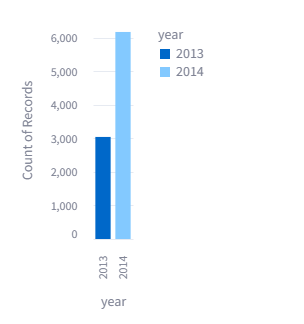
\includegraphics[height=150px]{grafica_anual.png} % Reemplaza con tu archivo real
		\caption{Número total de ventas de Kia por año}
		\label{fig:ejemplo_introduccion_grafico_anual}
	\end{minipage}
	\begin{minipage}{0.48\textwidth} % Ajusta el ancho según necesites
		\centering
		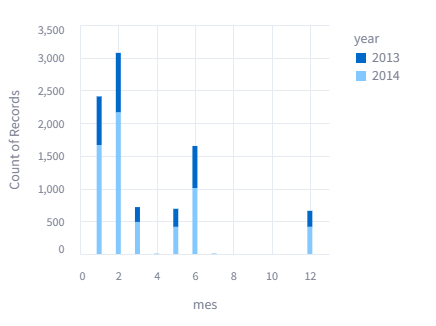
\includegraphics[height=150px]{grafica_mensual.png} % Reemplaza con tu archivo real
		\caption{Distribución de ventas de Kia por mes}
		\label{fig:ejemplo_introduccion_grafico_mensual}
	\end{minipage}
\end{figure}

Error detectado en la primera ejecución del código generado:
\textbf{\textit{Error message: Tz-aware datetime.datetime cannot be converted to datetime64 unless utc=True, at position 127}}

Posteriormente, al solicitar al modelo que genere la sección del reporte utilizando los datos obtenidos y estos gráficos, se muestra la primera sección del reporte en la columna principal. A partir de aquí, el resto de las secciones se generan de forma similar.

\begin{figure}[H] % Usamos h! para forzar la posición aquí si es necesario, pero considera htbp para más flexibilidad
	\centering % Centrar todo el conjunto de figuras horizontalmente
	\begin{minipage}{0.48\textwidth} % Ajusta el ancho según necesites (ej. 0.48 para dejar espacio entre figuras)
		\centering
		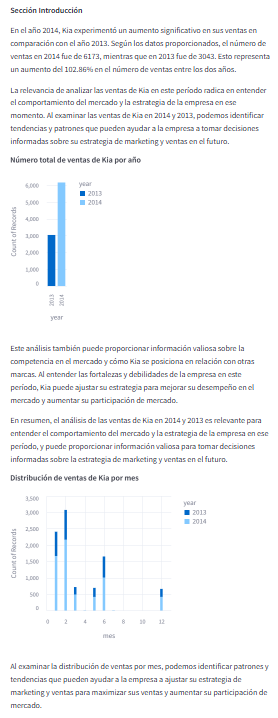
\includegraphics[height=\textheight]{intro.png} % Reemplaza con tu archivo real
		\caption{Sección Introducción}
		\label{fig:ejemplo_introduccion}
	\end{minipage}
\end{figure}


\section{Comparación de distintos modelos}

Para realizar una comparación de los distintos modelos disponibles, se generó un reporte para cada uno de ellos utilizando la misma consulta previamente analizada. A partir de estos reportes, se realizó una revisión para determinar su calidad. Para ello, se establecieron los siguientes criterios de comparación:

\begin{itemize}
	\item{Profundidad del Análisis:} Se analiza si el reporte va más allá de la simple presentación de datos, ofreciendo análisis e interpretaciones significativas.
	\item{Coherencia y Estructura:} El reporte está bien organizado y estructurado en secciones lógicas (Introducción, Datos 2013, Datos 2014, Comparación, Conclusiones).
	\item{Utilidad de las Visualizaciones:} ¿Son los gráficos y tablas relevantes y útiles para comprender los datos?
	\item{Precisión y Calidad General:} La información presentada en el reporte es precisa y se basa en los datos proporcionados. Demuestra una comprensión adecuada de la solicitud y los datos.
\end{itemize}

Para cada uno de estos criterios, se establecieron las siguientes clasificaciones:

\begin{itemize}
	\item{Alta:} En este aspecto, el reporte superó las expectativas.
	\item{Media:} El reporte cumple con las expectativas.
	\item{Baja:} El reporte contiene errores, inconsistencias o simplemente no alcanza el nivel esperado para este aspecto.
\end{itemize}

A partir de estos criterios y de una inspección manual y detallada de los reportes generados por el autor, se obtuvieron los siguientes resultados:

\begin{table}[htbp]
	\centering
	\caption{Comparación de Reportes de LLMs (Evaluación Manual)}
	\label{tab:comparacion_reportes}
	\begin{tabular}{@{}lccc@{}}
		\toprule
		Criterio & Llama3.3 & Mixtral-8x7b & Gemma2-9b \\
		\midrule
		Profundidad del Análisis & Alta & Media & Baja \\
		Coherencia y Estructura & Alta & Alta & Media \\
		Utilidad de las Visualizaciones & Media & Media & Baja \\
		Precisión y Calidad General & Alta & Alta & Media \\
		\bottomrule
	\end{tabular}
\end{table}

Para intentar automatizar este proceso de comparación de los reportes, así como para obtener una métrica más precisa, se utilizó un LLM más potente para calificar los mismos reportes. En este caso, se solicitó que se asignara una puntuación del uno al 100 en cada aspecto. Como modelo clasificatorio, se escogió Gemini-2.0-Flash-Thinking-Exp-01-21, debido a su amplio contexto (que permite entregarle los tres reportes a la vez) y su gran capacidad de razonamiento, lo que lo posiciona favorablemente en ChatBot Arena \cite{chiang2024chatbot}.

A partir de esta evaluación automatizada, se obtuvieron los siguientes resultados:

\begin{table}[htbp]
	\centering
	\caption{Comparación Automática de Reportes de LLMs (Evaluación con Gemini)}
	\label{tab:comparacion_reportes_gemini}
	\begin{tabular}{@{}lccc@{}}
		\toprule
		Criterio & Llama3.3 & Mixtral-8x7b & Gemma2-9b \\
		\midrule
		Profundidad del Análisis & 75 & 65 & 65 \\
		Coherencia y Estructura & 90 & 90 & 90 \\
		Utilidad de las Visualizaciones & 85 & 75 & 60 \\
		Precisión y Calidad General & 95 & 80 & 50 \\
		\bottomrule
	\end{tabular}
\end{table}
